\subsection{Casos de Prueba}
Este problema no tiene una gran variedad de casos particulares, debemos asegurarnos que se sigue el método de colocar un nuevo paquete en el camión con menos carga si es posible, y si no lo es que utiliza uno nuevo.\\
Los casos utilizados fueron:
\begin{itemize}
\item[•] un único paquete, como prueba base.
\item[•]6 paquetes cuya sumatoria de pesos no supera al límite de carga, para ver que no se utilicen camiones de más.
\item[•]2 casos donde se utiliza un camión por paquete.
\item[•]3 casos para comprobar que se intenta colocar paquetes en el camión con menor carga.
\end{itemize}

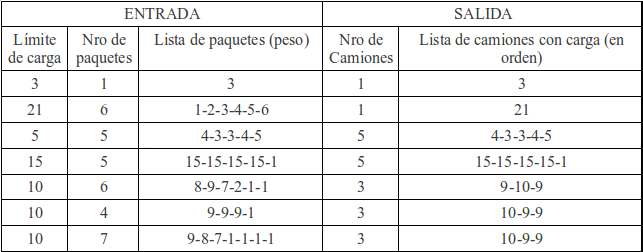
\includegraphics[scale=0.9]{ej1/Graficos/tablaPruebas.png} 